% Options for packages loaded elsewhere
\PassOptionsToPackage{unicode}{hyperref}
\PassOptionsToPackage{hyphens}{url}
%
\documentclass[
]{article}
\usepackage{amsmath,amssymb}
\usepackage{iftex}
\ifPDFTeX
  \usepackage[T1]{fontenc}
  \usepackage[utf8]{inputenc}
  \usepackage{textcomp} % provide euro and other symbols
\else % if luatex or xetex
  \usepackage{unicode-math} % this also loads fontspec
  \defaultfontfeatures{Scale=MatchLowercase}
  \defaultfontfeatures[\rmfamily]{Ligatures=TeX,Scale=1}
\fi
\usepackage{lmodern}
\ifPDFTeX\else
  % xetex/luatex font selection
\fi
% Use upquote if available, for straight quotes in verbatim environments
\IfFileExists{upquote.sty}{\usepackage{upquote}}{}
\IfFileExists{microtype.sty}{% use microtype if available
  \usepackage[]{microtype}
  \UseMicrotypeSet[protrusion]{basicmath} % disable protrusion for tt fonts
}{}
\makeatletter
\@ifundefined{KOMAClassName}{% if non-KOMA class
  \IfFileExists{parskip.sty}{%
    \usepackage{parskip}
  }{% else
    \setlength{\parindent}{0pt}
    \setlength{\parskip}{6pt plus 2pt minus 1pt}}
}{% if KOMA class
  \KOMAoptions{parskip=half}}
\makeatother
\usepackage{xcolor}
\usepackage[margin=1in]{geometry}
\usepackage{color}
\usepackage{fancyvrb}
\newcommand{\VerbBar}{|}
\newcommand{\VERB}{\Verb[commandchars=\\\{\}]}
\DefineVerbatimEnvironment{Highlighting}{Verbatim}{commandchars=\\\{\}}
% Add ',fontsize=\small' for more characters per line
\usepackage{framed}
\definecolor{shadecolor}{RGB}{248,248,248}
\newenvironment{Shaded}{\begin{snugshade}}{\end{snugshade}}
\newcommand{\AlertTok}[1]{\textcolor[rgb]{0.94,0.16,0.16}{#1}}
\newcommand{\AnnotationTok}[1]{\textcolor[rgb]{0.56,0.35,0.01}{\textbf{\textit{#1}}}}
\newcommand{\AttributeTok}[1]{\textcolor[rgb]{0.13,0.29,0.53}{#1}}
\newcommand{\BaseNTok}[1]{\textcolor[rgb]{0.00,0.00,0.81}{#1}}
\newcommand{\BuiltInTok}[1]{#1}
\newcommand{\CharTok}[1]{\textcolor[rgb]{0.31,0.60,0.02}{#1}}
\newcommand{\CommentTok}[1]{\textcolor[rgb]{0.56,0.35,0.01}{\textit{#1}}}
\newcommand{\CommentVarTok}[1]{\textcolor[rgb]{0.56,0.35,0.01}{\textbf{\textit{#1}}}}
\newcommand{\ConstantTok}[1]{\textcolor[rgb]{0.56,0.35,0.01}{#1}}
\newcommand{\ControlFlowTok}[1]{\textcolor[rgb]{0.13,0.29,0.53}{\textbf{#1}}}
\newcommand{\DataTypeTok}[1]{\textcolor[rgb]{0.13,0.29,0.53}{#1}}
\newcommand{\DecValTok}[1]{\textcolor[rgb]{0.00,0.00,0.81}{#1}}
\newcommand{\DocumentationTok}[1]{\textcolor[rgb]{0.56,0.35,0.01}{\textbf{\textit{#1}}}}
\newcommand{\ErrorTok}[1]{\textcolor[rgb]{0.64,0.00,0.00}{\textbf{#1}}}
\newcommand{\ExtensionTok}[1]{#1}
\newcommand{\FloatTok}[1]{\textcolor[rgb]{0.00,0.00,0.81}{#1}}
\newcommand{\FunctionTok}[1]{\textcolor[rgb]{0.13,0.29,0.53}{\textbf{#1}}}
\newcommand{\ImportTok}[1]{#1}
\newcommand{\InformationTok}[1]{\textcolor[rgb]{0.56,0.35,0.01}{\textbf{\textit{#1}}}}
\newcommand{\KeywordTok}[1]{\textcolor[rgb]{0.13,0.29,0.53}{\textbf{#1}}}
\newcommand{\NormalTok}[1]{#1}
\newcommand{\OperatorTok}[1]{\textcolor[rgb]{0.81,0.36,0.00}{\textbf{#1}}}
\newcommand{\OtherTok}[1]{\textcolor[rgb]{0.56,0.35,0.01}{#1}}
\newcommand{\PreprocessorTok}[1]{\textcolor[rgb]{0.56,0.35,0.01}{\textit{#1}}}
\newcommand{\RegionMarkerTok}[1]{#1}
\newcommand{\SpecialCharTok}[1]{\textcolor[rgb]{0.81,0.36,0.00}{\textbf{#1}}}
\newcommand{\SpecialStringTok}[1]{\textcolor[rgb]{0.31,0.60,0.02}{#1}}
\newcommand{\StringTok}[1]{\textcolor[rgb]{0.31,0.60,0.02}{#1}}
\newcommand{\VariableTok}[1]{\textcolor[rgb]{0.00,0.00,0.00}{#1}}
\newcommand{\VerbatimStringTok}[1]{\textcolor[rgb]{0.31,0.60,0.02}{#1}}
\newcommand{\WarningTok}[1]{\textcolor[rgb]{0.56,0.35,0.01}{\textbf{\textit{#1}}}}
\usepackage{longtable,booktabs,array}
\usepackage{calc} % for calculating minipage widths
% Correct order of tables after \paragraph or \subparagraph
\usepackage{etoolbox}
\makeatletter
\patchcmd\longtable{\par}{\if@noskipsec\mbox{}\fi\par}{}{}
\makeatother
% Allow footnotes in longtable head/foot
\IfFileExists{footnotehyper.sty}{\usepackage{footnotehyper}}{\usepackage{footnote}}
\makesavenoteenv{longtable}
\usepackage{graphicx}
\makeatletter
\def\maxwidth{\ifdim\Gin@nat@width>\linewidth\linewidth\else\Gin@nat@width\fi}
\def\maxheight{\ifdim\Gin@nat@height>\textheight\textheight\else\Gin@nat@height\fi}
\makeatother
% Scale images if necessary, so that they will not overflow the page
% margins by default, and it is still possible to overwrite the defaults
% using explicit options in \includegraphics[width, height, ...]{}
\setkeys{Gin}{width=\maxwidth,height=\maxheight,keepaspectratio}
% Set default figure placement to htbp
\makeatletter
\def\fps@figure{htbp}
\makeatother
\setlength{\emergencystretch}{3em} % prevent overfull lines
\providecommand{\tightlist}{%
  \setlength{\itemsep}{0pt}\setlength{\parskip}{0pt}}
\setcounter{secnumdepth}{5}
\usepackage{booktabs}
\ifLuaTeX
  \usepackage{selnolig}  % disable illegal ligatures
\fi
\usepackage[]{natbib}
\bibliographystyle{apalike}
\IfFileExists{bookmark.sty}{\usepackage{bookmark}}{\usepackage{hyperref}}
\IfFileExists{xurl.sty}{\usepackage{xurl}}{} % add URL line breaks if available
\urlstyle{same}
\hypersetup{
  pdftitle={Homeworks for James' Stats classes},
  pdfauthor={Zhifei Yu},
  hidelinks,
  pdfcreator={LaTeX via pandoc}}

\title{Homeworks for James' Stats classes}
\author{Zhifei Yu}
\date{2023-7-14}

\begin{document}
\maketitle

{
\setcounter{tocdepth}{2}
\tableofcontents
}
\hypertarget{welcome}{%
\section*{Welcome!}\label{welcome}}
\addcontentsline{toc}{section}{Welcome!}

Howdy! This is a collection of 4 assignments from James Scott's probability and Statistics courses, written by Zhifei Yu a.k.a Kevin.

\hypertarget{homework-1}{%
\section{Homework 1}\label{homework-1}}

\begin{Shaded}
\begin{Highlighting}[]
\FunctionTok{library}\NormalTok{(tidyverse)}
\FunctionTok{library}\NormalTok{(knitr)}
\FunctionTok{library}\NormalTok{(pander)}
\end{Highlighting}
\end{Shaded}

\hypertarget{problem-1-playlists-revisited}{%
\subsection{Problem 1 Playlists revisited}\label{problem-1-playlists-revisited}}

\begin{Shaded}
\begin{Highlighting}[]
\NormalTok{playlist }\OtherTok{=} \FunctionTok{read.csv}\NormalTok{(}\StringTok{\textquotesingle{}/Users/kevin/Academic/MAE/2023 Summer/R\&Prob\&Stat/Assignments/Data/plays\_top50.csv\textquotesingle{}}\NormalTok{,}\AttributeTok{header =} \ConstantTok{TRUE}\NormalTok{)}
\end{Highlighting}
\end{Shaded}

\hypertarget{part-a}{%
\subsubsection{Part A}\label{part-a}}

\begin{Shaded}
\begin{Highlighting}[]
\FunctionTok{xtabs}\NormalTok{(}\SpecialCharTok{\textasciitilde{}}\NormalTok{ daft.punk }\SpecialCharTok{+}\NormalTok{ david.bowie, }\AttributeTok{data=}\NormalTok{playlist,}\AttributeTok{sparse=}\ConstantTok{FALSE}\NormalTok{) }\SpecialCharTok{\%\textgreater{}\%} \FunctionTok{prop.table}\NormalTok{(}\DecValTok{2}\NormalTok{) }\SpecialCharTok{\%\textgreater{}\%} \FunctionTok{round}\NormalTok{(}\DecValTok{3}\NormalTok{) }\SpecialCharTok{\%\textgreater{}\%} \FunctionTok{pander}\NormalTok{()}
\end{Highlighting}
\end{Shaded}

\begin{longtable}[]{@{}
  >{\centering\arraybackslash}p{(\columnwidth - 4\tabcolsep) * \real{0.1250}}
  >{\centering\arraybackslash}p{(\columnwidth - 4\tabcolsep) * \real{0.1111}}
  >{\centering\arraybackslash}p{(\columnwidth - 4\tabcolsep) * \real{0.1111}}@{}}
\toprule\noalign{}
\begin{minipage}[b]{\linewidth}\centering
~
\end{minipage} & \begin{minipage}[b]{\linewidth}\centering
0
\end{minipage} & \begin{minipage}[b]{\linewidth}\centering
1
\end{minipage} \\
\midrule\noalign{}
\endhead
\bottomrule\noalign{}
\endlastfoot
\textbf{0} & 0.925 & 0.912 \\
\textbf{1} & 0.075 & 0.088 \\
\end{longtable}

Column:

0: never plays Daft Punk

1: plays Daft Punk

Row:

0: never plays David Bowie

1: plays David Bowie

\hypertarget{part-b}{%
\subsubsection{Part B}\label{part-b}}

To check out if 2 events are independent, we can use the definition: If A and B are independent, then P(A\textbar B) = P(A\textbar\textasciitilde B) = P(A) To make it clear, ``plays Pink Floyd'' is considered as event B, ``plays Johnny cash'' is event A.

\begin{Shaded}
\begin{Highlighting}[]
\FunctionTok{xtabs}\NormalTok{(}\SpecialCharTok{\textasciitilde{}}\NormalTok{ johnny.cash, }\AttributeTok{data=}\NormalTok{playlist,}\AttributeTok{sparse=}\ConstantTok{FALSE}\NormalTok{) }\SpecialCharTok{\%\textgreater{}\%} \FunctionTok{prop.table}\NormalTok{() }\SpecialCharTok{\%\textgreater{}\%} \FunctionTok{round}\NormalTok{(}\DecValTok{3}\NormalTok{) }\SpecialCharTok{\%\textgreater{}\%} \FunctionTok{pander}\NormalTok{()}
\end{Highlighting}
\end{Shaded}

\begin{longtable}[]{@{}
  >{\centering\arraybackslash}p{(\columnwidth - 2\tabcolsep) * \real{0.0972}}
  >{\centering\arraybackslash}p{(\columnwidth - 2\tabcolsep) * \real{0.0972}}@{}}
\toprule\noalign{}
\begin{minipage}[b]{\linewidth}\centering
0
\end{minipage} & \begin{minipage}[b]{\linewidth}\centering
1
\end{minipage} \\
\midrule\noalign{}
\endhead
\bottomrule\noalign{}
\endlastfoot
0.94 & 0.06 \\
\end{longtable}

0: never plays Johnny Cash

1: plays Johnny Cash

\begin{Shaded}
\begin{Highlighting}[]
\FunctionTok{xtabs}\NormalTok{(}\SpecialCharTok{\textasciitilde{}}\NormalTok{ johnny.cash }\SpecialCharTok{+}\NormalTok{ pink.floyd, }\AttributeTok{data=}\NormalTok{playlist,}\AttributeTok{sparse=}\ConstantTok{FALSE}\NormalTok{) }\SpecialCharTok{\%\textgreater{}\%} \FunctionTok{prop.table}\NormalTok{(}\DecValTok{2}\NormalTok{) }\SpecialCharTok{\%\textgreater{}\%} \FunctionTok{round}\NormalTok{(}\DecValTok{3}\NormalTok{) }\SpecialCharTok{\%\textgreater{}\%} \FunctionTok{pander}\NormalTok{()}
\end{Highlighting}
\end{Shaded}

\begin{longtable}[]{@{}
  >{\centering\arraybackslash}p{(\columnwidth - 4\tabcolsep) * \real{0.1250}}
  >{\centering\arraybackslash}p{(\columnwidth - 4\tabcolsep) * \real{0.1111}}
  >{\centering\arraybackslash}p{(\columnwidth - 4\tabcolsep) * \real{0.1111}}@{}}
\toprule\noalign{}
\begin{minipage}[b]{\linewidth}\centering
~
\end{minipage} & \begin{minipage}[b]{\linewidth}\centering
0
\end{minipage} & \begin{minipage}[b]{\linewidth}\centering
1
\end{minipage} \\
\midrule\noalign{}
\endhead
\bottomrule\noalign{}
\endlastfoot
\textbf{0} & 0.945 & 0.895 \\
\textbf{1} & 0.055 & 0.105 \\
\end{longtable}

Column:

0: never plays Johnny Cash

1: plays Johnny Cash

Row:

0: never plays Pink Floyd

1: plays Pink Floyd

So, in this case P(A) = 6\%, P(A\textbar B) = 10.5\%, P(A\textbar not B) = 5.5\%; clearly, they are not equal. Therefore, they are not independent and seem to have positive relationship.

Or we can check it by if P(B) = P(B\textbar A) = P(B\textbar\textasciitilde A)

\begin{Shaded}
\begin{Highlighting}[]
\FunctionTok{xtabs}\NormalTok{(}\SpecialCharTok{\textasciitilde{}}\NormalTok{ pink.floyd, }\AttributeTok{data=}\NormalTok{playlist,}\AttributeTok{sparse=}\ConstantTok{FALSE}\NormalTok{) }\SpecialCharTok{\%\textgreater{}\%} \FunctionTok{prop.table}\NormalTok{() }\SpecialCharTok{\%\textgreater{}\%} \FunctionTok{round}\NormalTok{(}\DecValTok{3}\NormalTok{) }\SpecialCharTok{\%\textgreater{}\%} \FunctionTok{pander}\NormalTok{() }\SpecialCharTok{\%\textgreater{}\%} \FunctionTok{pander}\NormalTok{()}
\end{Highlighting}
\end{Shaded}

\begin{longtable}[]{@{}
  >{\centering\arraybackslash}p{(\columnwidth - 2\tabcolsep) * \real{0.1111}}
  >{\centering\arraybackslash}p{(\columnwidth - 2\tabcolsep) * \real{0.1111}}@{}}
\toprule\noalign{}
\begin{minipage}[b]{\linewidth}\centering
0
\end{minipage} & \begin{minipage}[b]{\linewidth}\centering
1
\end{minipage} \\
\midrule\noalign{}
\endhead
\bottomrule\noalign{}
\endlastfoot
0.895 & 0.105 \\
\end{longtable}

0: never plays Pink Floyd

1: plays Pink Floyd

\begin{Shaded}
\begin{Highlighting}[]
\FunctionTok{xtabs}\NormalTok{(}\SpecialCharTok{\textasciitilde{}}\NormalTok{ pink.floyd }\SpecialCharTok{+}\NormalTok{ johnny.cash, }\AttributeTok{data=}\NormalTok{playlist,}\AttributeTok{sparse=}\ConstantTok{FALSE}\NormalTok{) }\SpecialCharTok{\%\textgreater{}\%} \FunctionTok{prop.table}\NormalTok{(}\DecValTok{2}\NormalTok{) }\SpecialCharTok{\%\textgreater{}\%} \FunctionTok{round}\NormalTok{(}\DecValTok{3}\NormalTok{) }\SpecialCharTok{\%\textgreater{}\%} \FunctionTok{pander}\NormalTok{()}
\end{Highlighting}
\end{Shaded}

\begin{longtable}[]{@{}
  >{\centering\arraybackslash}p{(\columnwidth - 4\tabcolsep) * \real{0.1250}}
  >{\centering\arraybackslash}p{(\columnwidth - 4\tabcolsep) * \real{0.0833}}
  >{\centering\arraybackslash}p{(\columnwidth - 4\tabcolsep) * \real{0.1111}}@{}}
\toprule\noalign{}
\begin{minipage}[b]{\linewidth}\centering
~
\end{minipage} & \begin{minipage}[b]{\linewidth}\centering
0
\end{minipage} & \begin{minipage}[b]{\linewidth}\centering
1
\end{minipage} \\
\midrule\noalign{}
\endhead
\bottomrule\noalign{}
\endlastfoot
\textbf{0} & 0.9 & 0.817 \\
\textbf{1} & 0.1 & 0.183 \\
\end{longtable}

Column:

0: never plays Pink Floyd

1: plays Pink Floyd

Row:

0: never plays Johnny Cash

1: plays Johnny Cash

Clearly, P(B) = 10.5\%, P(B\textbar A) = 18.3\%, and P(B\textbar\textasciitilde A) = 10\%, so they are not close to each other.

\hypertarget{problem-2-super-bowl-ads}{%
\subsection{Problem 2 Super Bowl ads}\label{problem-2-super-bowl-ads}}

\begin{Shaded}
\begin{Highlighting}[]
\NormalTok{superbowl }\OtherTok{=} \FunctionTok{read.csv}\NormalTok{(}\StringTok{\textquotesingle{}/Users/kevin/Academic/MAE/2023 Summer/R\&Prob\&Stat/Assignments/Data/superbowl.csv\textquotesingle{}}\NormalTok{,}\AttributeTok{header =} \ConstantTok{TRUE}\NormalTok{)}
\end{Highlighting}
\end{Shaded}

\hypertarget{part-a-1}{%
\subsubsection{Part A}\label{part-a-1}}

\begin{Shaded}
\begin{Highlighting}[]
\FunctionTok{xtabs}\NormalTok{(}\SpecialCharTok{\textasciitilde{}}\NormalTok{ danger, }\AttributeTok{data=}\NormalTok{superbowl,}\AttributeTok{sparse=}\ConstantTok{FALSE}\NormalTok{) }\SpecialCharTok{\%\textgreater{}\%} \FunctionTok{prop.table}\NormalTok{() }\SpecialCharTok{\%\textgreater{}\%} \FunctionTok{round}\NormalTok{(}\DecValTok{2}\NormalTok{) }\SpecialCharTok{\%\textgreater{}\%} \FunctionTok{pander}\NormalTok{()}
\end{Highlighting}
\end{Shaded}

\begin{longtable}[]{@{}
  >{\centering\arraybackslash}p{(\columnwidth - 2\tabcolsep) * \real{0.1111}}
  >{\centering\arraybackslash}p{(\columnwidth - 2\tabcolsep) * \real{0.1111}}@{}}
\toprule\noalign{}
\begin{minipage}[b]{\linewidth}\centering
FALSE
\end{minipage} & \begin{minipage}[b]{\linewidth}\centering
TRUE
\end{minipage} \\
\midrule\noalign{}
\endhead
\bottomrule\noalign{}
\endlastfoot
0.7 & 0.3 \\
\end{longtable}

True: should be danger

False: not danger

Which returns the results that P(danger = TRUE) = 30\%

\begin{Shaded}
\begin{Highlighting}[]
\FunctionTok{xtabs}\NormalTok{(}\SpecialCharTok{\textasciitilde{}}\NormalTok{ danger }\SpecialCharTok{+}\NormalTok{ funny, }\AttributeTok{data=}\NormalTok{superbowl,}\AttributeTok{sparse=}\ConstantTok{FALSE}\NormalTok{) }\SpecialCharTok{\%\textgreater{}\%} \FunctionTok{prop.table}\NormalTok{(}\DecValTok{2}\NormalTok{) }\SpecialCharTok{\%\textgreater{}\%} \FunctionTok{round}\NormalTok{(}\DecValTok{2}\NormalTok{) }\SpecialCharTok{\%\textgreater{}\%} \FunctionTok{pander}\NormalTok{()}
\end{Highlighting}
\end{Shaded}

\begin{longtable}[]{@{}
  >{\centering\arraybackslash}p{(\columnwidth - 4\tabcolsep) * \real{0.1667}}
  >{\centering\arraybackslash}p{(\columnwidth - 4\tabcolsep) * \real{0.1111}}
  >{\centering\arraybackslash}p{(\columnwidth - 4\tabcolsep) * \real{0.1111}}@{}}
\toprule\noalign{}
\begin{minipage}[b]{\linewidth}\centering
~
\end{minipage} & \begin{minipage}[b]{\linewidth}\centering
FALSE
\end{minipage} & \begin{minipage}[b]{\linewidth}\centering
TRUE
\end{minipage} \\
\midrule\noalign{}
\endhead
\bottomrule\noalign{}
\endlastfoot
\textbf{FALSE} & 0.88 & 0.61 \\
\textbf{TRUE} & 0.12 & 0.39 \\
\end{longtable}

Column:

True: should be danger

False: not danger

Row:

True: should be funny

False: not funny

From the table, we can know that:

P(danger = TRUE \textbar{} funny = TRUE) = 39\%

P(danger = TRUE \textbar{} funny = FALSE) = 12\%

Undoubtedly, from this statistics, humor and danger are absolutely not independent because P(danger) ≠ P(danger\textbar funny) ≠ P(danger\textbar not funny)

It seems that humor are indeed more or less a indication of danger for this ads, because under the condition that ads are funny, the probability of danger seems to be higher than unconditional probability and under the another condition that ads are not funny, the probability of it shows way much lower than unconditional probability.

\hypertarget{part-b-1}{%
\subsubsection{Part B}\label{part-b-1}}

\begin{Shaded}
\begin{Highlighting}[]
\FunctionTok{xtabs}\NormalTok{(}\SpecialCharTok{\textasciitilde{}}\NormalTok{ animals, }\AttributeTok{data=}\NormalTok{superbowl,}\AttributeTok{sparse=}\ConstantTok{FALSE}\NormalTok{) }\SpecialCharTok{\%\textgreater{}\%} \FunctionTok{prop.table}\NormalTok{() }\SpecialCharTok{\%\textgreater{}\%} \FunctionTok{round}\NormalTok{(}\DecValTok{2}\NormalTok{) }\SpecialCharTok{\%\textgreater{}\%} \FunctionTok{pander}\NormalTok{()}
\end{Highlighting}
\end{Shaded}

\begin{longtable}[]{@{}
  >{\centering\arraybackslash}p{(\columnwidth - 2\tabcolsep) * \real{0.1111}}
  >{\centering\arraybackslash}p{(\columnwidth - 2\tabcolsep) * \real{0.1111}}@{}}
\toprule\noalign{}
\begin{minipage}[b]{\linewidth}\centering
FALSE
\end{minipage} & \begin{minipage}[b]{\linewidth}\centering
TRUE
\end{minipage} \\
\midrule\noalign{}
\endhead
\bottomrule\noalign{}
\endlastfoot
0.63 & 0.37 \\
\end{longtable}

True: with animals False: without animals

Which returns the results that P(animals = TRUE) = 37\%

\begin{Shaded}
\begin{Highlighting}[]
\FunctionTok{xtabs}\NormalTok{(}\SpecialCharTok{\textasciitilde{}}\NormalTok{ animals }\SpecialCharTok{+}\NormalTok{ use\_sex, }\AttributeTok{data=}\NormalTok{superbowl,}\AttributeTok{sparse=}\ConstantTok{FALSE}\NormalTok{) }\SpecialCharTok{\%\textgreater{}\%} \FunctionTok{prop.table}\NormalTok{(}\DecValTok{2}\NormalTok{) }\SpecialCharTok{\%\textgreater{}\%} \FunctionTok{round}\NormalTok{(}\DecValTok{2}\NormalTok{) }\SpecialCharTok{\%\textgreater{}\%} \FunctionTok{pander}\NormalTok{()}
\end{Highlighting}
\end{Shaded}

\begin{longtable}[]{@{}
  >{\centering\arraybackslash}p{(\columnwidth - 4\tabcolsep) * \real{0.1667}}
  >{\centering\arraybackslash}p{(\columnwidth - 4\tabcolsep) * \real{0.1111}}
  >{\centering\arraybackslash}p{(\columnwidth - 4\tabcolsep) * \real{0.1111}}@{}}
\toprule\noalign{}
\begin{minipage}[b]{\linewidth}\centering
~
\end{minipage} & \begin{minipage}[b]{\linewidth}\centering
FALSE
\end{minipage} & \begin{minipage}[b]{\linewidth}\centering
TRUE
\end{minipage} \\
\midrule\noalign{}
\endhead
\bottomrule\noalign{}
\endlastfoot
\textbf{FALSE} & 0.63 & 0.62 \\
\textbf{TRUE} & 0.37 & 0.38 \\
\end{longtable}

Column:

True: with animals

False: without animals

Row:

True: has sex contents

False: not have sex contents

From the table, we can know that:

P(animals = TRUE \textbar{} use\_sex = TRUE) = 38\%

P(animals = TRUE \textbar{} use\_sex = FALSE) = 37\%

From the probability tables and unconditional probability, I think animals and use\_sex are statistically independent.My argument is that the unconditional probability of animals seems to be very close to the conditional probabilities on both conditions that using sex and not using, which, from definition, shows this 2 events are independent.

\hypertarget{part-c}{%
\subsubsection{Part C}\label{part-c}}

\begin{Shaded}
\begin{Highlighting}[]
\FunctionTok{xtabs}\NormalTok{(}\SpecialCharTok{\textasciitilde{}}\NormalTok{ celebrity, }\AttributeTok{data=}\NormalTok{superbowl,}\AttributeTok{sparse=}\ConstantTok{FALSE}\NormalTok{) }\SpecialCharTok{\%\textgreater{}\%} \FunctionTok{prop.table}\NormalTok{() }\SpecialCharTok{\%\textgreater{}\%} \FunctionTok{round}\NormalTok{(}\DecValTok{2}\NormalTok{) }\SpecialCharTok{\%\textgreater{}\%} \FunctionTok{pander}\NormalTok{()}
\end{Highlighting}
\end{Shaded}

\begin{longtable}[]{@{}
  >{\centering\arraybackslash}p{(\columnwidth - 2\tabcolsep) * \real{0.1111}}
  >{\centering\arraybackslash}p{(\columnwidth - 2\tabcolsep) * \real{0.1111}}@{}}
\toprule\noalign{}
\begin{minipage}[b]{\linewidth}\centering
FALSE
\end{minipage} & \begin{minipage}[b]{\linewidth}\centering
TRUE
\end{minipage} \\
\midrule\noalign{}
\endhead
\bottomrule\noalign{}
\endlastfoot
0.71 & 0.29 \\
\end{longtable}

True: with celebrities

False: without celebrities

Which returns the results that P(celebrity = TRUE) = 29\%

\begin{Shaded}
\begin{Highlighting}[]
\FunctionTok{xtabs}\NormalTok{(}\SpecialCharTok{\textasciitilde{}}\NormalTok{ celebrity }\SpecialCharTok{+}\NormalTok{ patriotic, }\AttributeTok{data=}\NormalTok{superbowl,}\AttributeTok{sparse=}\ConstantTok{FALSE}\NormalTok{) }\SpecialCharTok{\%\textgreater{}\%} \FunctionTok{prop.table}\NormalTok{(}\DecValTok{2}\NormalTok{) }\SpecialCharTok{\%\textgreater{}\%} \FunctionTok{round}\NormalTok{(}\DecValTok{2}\NormalTok{) }\SpecialCharTok{\%\textgreater{}\%} \FunctionTok{pander}\NormalTok{()}
\end{Highlighting}
\end{Shaded}

\begin{longtable}[]{@{}
  >{\centering\arraybackslash}p{(\columnwidth - 4\tabcolsep) * \real{0.1667}}
  >{\centering\arraybackslash}p{(\columnwidth - 4\tabcolsep) * \real{0.1111}}
  >{\centering\arraybackslash}p{(\columnwidth - 4\tabcolsep) * \real{0.1111}}@{}}
\toprule\noalign{}
\begin{minipage}[b]{\linewidth}\centering
~
\end{minipage} & \begin{minipage}[b]{\linewidth}\centering
FALSE
\end{minipage} & \begin{minipage}[b]{\linewidth}\centering
TRUE
\end{minipage} \\
\midrule\noalign{}
\endhead
\bottomrule\noalign{}
\endlastfoot
\textbf{FALSE} & 0.71 & 0.71 \\
\textbf{TRUE} & 0.29 & 0.29 \\
\end{longtable}

Column:

True: with celebrities

False: without celebrities

Row:

True: has patriotic contents

False: not have patriotic contents

From the table, we can know that:

P(celebrity = TRUE \textbar{} patriotic = TRUE) = 29\%

P(celebrity = TRUE \textbar{} patriotic = FALSE) = 29\%

Similar with Part B, in this part, the unconditional probability of celebrity is nearly equal to the 2 conditional probabilities of both showing patriotic contents and not showing this. Thus, they are independent on the basis of this data.

\hypertarget{problem-3-beauty-or-not-in-the-classroom}{%
\subsection{Problem 3 Beauty, or not, in the classroom}\label{problem-3-beauty-or-not-in-the-classroom}}

\begin{Shaded}
\begin{Highlighting}[]
\FunctionTok{library}\NormalTok{(ggplot2)}
\NormalTok{profs }\OtherTok{=} \FunctionTok{read.csv}\NormalTok{(}\StringTok{\textquotesingle{}/Users/kevin/Academic/MAE/2023 Summer/R\&Prob\&Stat/Assignments/Data/profs.csv\textquotesingle{}}\NormalTok{,}\AttributeTok{header =} \ConstantTok{TRUE}\NormalTok{)}
\end{Highlighting}
\end{Shaded}

\hypertarget{part-a-2}{%
\subsubsection{Part A}\label{part-a-2}}

\begin{Shaded}
\begin{Highlighting}[]
\FunctionTok{ggplot}\NormalTok{(profs,}\FunctionTok{aes}\NormalTok{(}\AttributeTok{x=}\NormalTok{eval)) }\SpecialCharTok{+} \FunctionTok{geom\_histogram}\NormalTok{(}\AttributeTok{bins=}\DecValTok{20}\NormalTok{,}\AttributeTok{color=}\StringTok{"black"}\NormalTok{, }\AttributeTok{fill=}\StringTok{"white"}\NormalTok{) }\SpecialCharTok{+} \FunctionTok{ggtitle}\NormalTok{(}\StringTok{\textquotesingle{}Evaluation Scores Distribution\textquotesingle{}}\NormalTok{) }\SpecialCharTok{+} \FunctionTok{labs}\NormalTok{(}\AttributeTok{x =} \StringTok{"Evaluation Scores"}\NormalTok{, }\AttributeTok{y =} \StringTok{"Count"}\NormalTok{)}
\end{Highlighting}
\end{Shaded}

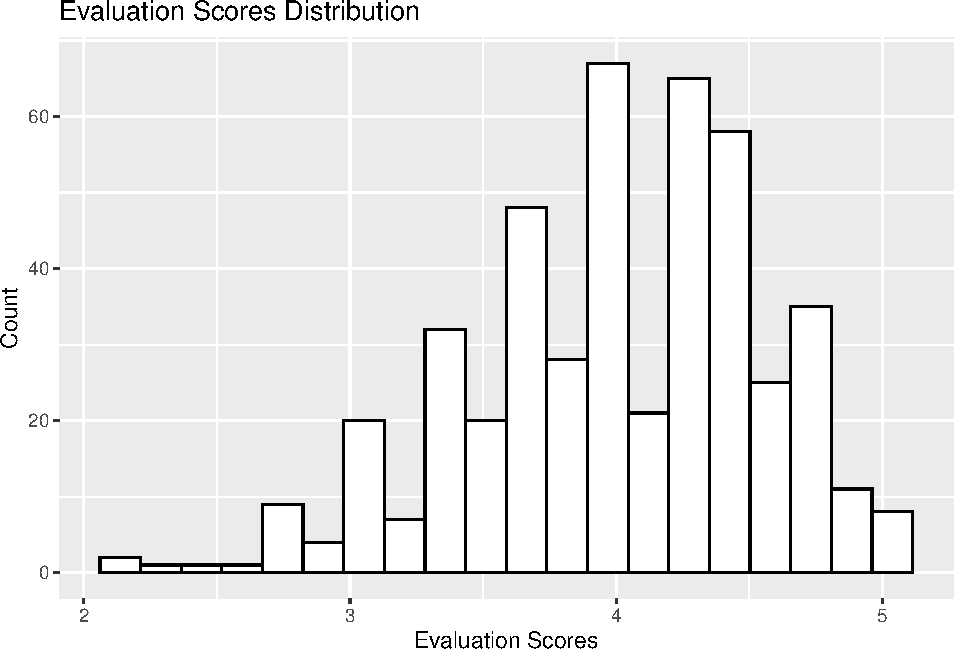
\includegraphics{_main_files/figure-latex/unnamed-chunk-17-1.pdf}

Above is the histogram plot that shows course evaluation scores of all professors.

X axis shows the evaluation scores which professors have gained.

Y axis shows tha counting of each score.

We can see around 4 is where the most scores are sited. So I guess that most UT's professor are pretty good so that they can get good evaluations scores from students.

\hypertarget{part-b-2}{%
\subsubsection{Part B}\label{part-b-2}}

\begin{Shaded}
\begin{Highlighting}[]
\FunctionTok{ggplot}\NormalTok{(profs, }\FunctionTok{aes}\NormalTok{(}\AttributeTok{x=}\NormalTok{native, }\AttributeTok{y=}\NormalTok{eval, }\AttributeTok{fill=}\NormalTok{native)) }\SpecialCharTok{+} \FunctionTok{geom\_boxplot}\NormalTok{() }\SpecialCharTok{+} \FunctionTok{ggtitle}\NormalTok{(}\StringTok{\textquotesingle{}Scores by whether native speaker or not\textquotesingle{}}\NormalTok{) }\SpecialCharTok{+} \FunctionTok{labs}\NormalTok{(}\AttributeTok{x =} \StringTok{"Native Speaker"}\NormalTok{, }\AttributeTok{y =} \StringTok{"Evaluation Scores"}\NormalTok{)}
\end{Highlighting}
\end{Shaded}

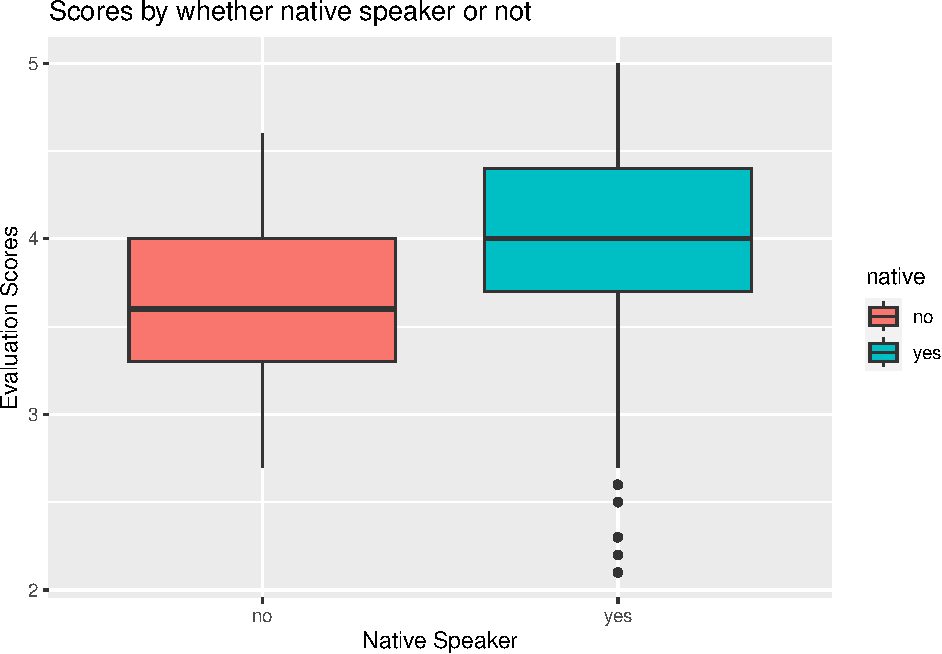
\includegraphics{_main_files/figure-latex/unnamed-chunk-18-1.pdf}

The left red box represents the non-native English speaker.

The right blue box stands for native speaker. Y axis means the evaluation scores.

So, from this boxplot, we can conclude that native speakers generally get better score than non-native speaker.

\hypertarget{part-c-1}{%
\subsubsection{Part C}\label{part-c-1}}

\begin{Shaded}
\begin{Highlighting}[]
\FunctionTok{ggplot}\NormalTok{(profs,}\FunctionTok{aes}\NormalTok{(}\AttributeTok{x=}\NormalTok{eval)) }\SpecialCharTok{+} \FunctionTok{geom\_histogram}\NormalTok{(}\AttributeTok{bins =} \DecValTok{20}\NormalTok{,}\AttributeTok{color=}\StringTok{"green"}\NormalTok{, }\AttributeTok{fill=}\StringTok{"grey"}\NormalTok{) }\SpecialCharTok{+} \FunctionTok{ggtitle}\NormalTok{(}\StringTok{\textquotesingle{}Evaluation Scores Distribution by gender\textquotesingle{}}\NormalTok{) }\SpecialCharTok{+} \FunctionTok{facet\_grid}\NormalTok{(.}\SpecialCharTok{\textasciitilde{}}\NormalTok{gender) }\SpecialCharTok{+} \FunctionTok{labs}\NormalTok{(}\AttributeTok{x =} \StringTok{"Evaluation Scores"}\NormalTok{, }\AttributeTok{y =} \StringTok{"Count"}\NormalTok{)}
\end{Highlighting}
\end{Shaded}

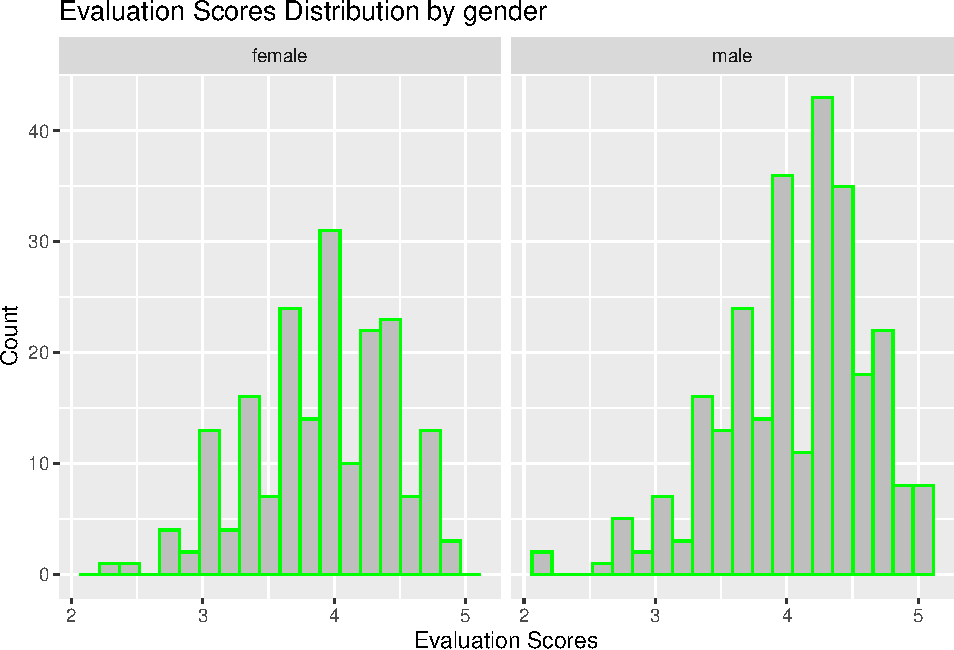
\includegraphics{_main_files/figure-latex/unnamed-chunk-19-1.pdf}

From this plot, we can see that male professors are more focused around 4, whereas female professors are more spread-out.

\hypertarget{part-d}{%
\subsubsection{Part D}\label{part-d}}

\begin{Shaded}
\begin{Highlighting}[]
\FunctionTok{ggplot}\NormalTok{(profs, }\FunctionTok{aes}\NormalTok{(}\AttributeTok{x=}\NormalTok{beauty, }\AttributeTok{y=}\NormalTok{eval)) }\SpecialCharTok{+} \FunctionTok{geom\_point}\NormalTok{() }\SpecialCharTok{+} \FunctionTok{ggtitle}\NormalTok{(}\StringTok{\textquotesingle{}Scores Distribution by Beauty\textquotesingle{}}\NormalTok{) }\SpecialCharTok{+} \FunctionTok{labs}\NormalTok{(}\AttributeTok{x =} \StringTok{"Physical Attractness"}\NormalTok{, }\AttributeTok{y =} \StringTok{"Evaluation Scores"}\NormalTok{)}
\end{Highlighting}
\end{Shaded}

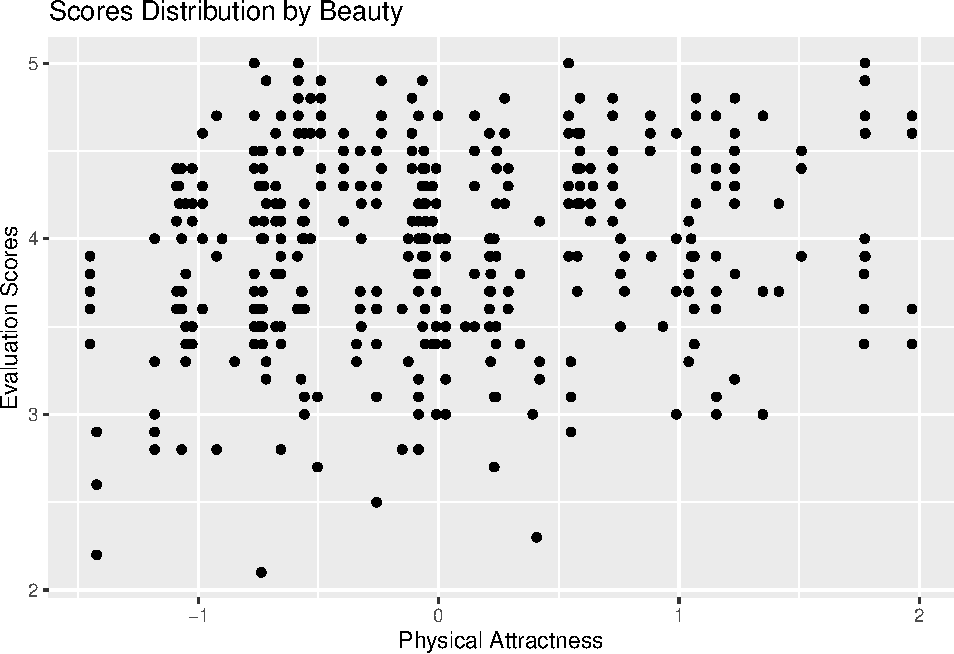
\includegraphics{_main_files/figure-latex/unnamed-chunk-20-1.pdf}

X axis stands for the score of beauty.

I think that the physical attraction basically has slightly positive relationship with evaluation scores but cannot be a predictive indicator of evaluation.

\hypertarget{problem-4-sat-scores-for-ut-students}{%
\subsection{Problem 4 SAT scores for UT students}\label{problem-4-sat-scores-for-ut-students}}

\begin{Shaded}
\begin{Highlighting}[]
\NormalTok{utsat }\OtherTok{=} \FunctionTok{read.csv}\NormalTok{(}\StringTok{\textquotesingle{}/Users/kevin/Academic/MAE/2023 Summer/R\&Prob\&Stat/Assignments/Data/utsat.csv\textquotesingle{}}\NormalTok{,}\AttributeTok{header =} \ConstantTok{TRUE}\NormalTok{)}
\NormalTok{tb }\OtherTok{=} \FunctionTok{data.frame}\NormalTok{(}\AttributeTok{Scores =} \FunctionTok{c}\NormalTok{(}\StringTok{"SAT{-}V"}\NormalTok{, }\StringTok{"SAT{-}Q"}\NormalTok{, }\StringTok{"GPA"}\NormalTok{),}
                \AttributeTok{Mean =} \FunctionTok{c}\NormalTok{(}\FunctionTok{mean}\NormalTok{(utsat}\SpecialCharTok{$}\NormalTok{SAT.V), }\FunctionTok{mean}\NormalTok{(utsat}\SpecialCharTok{$}\NormalTok{SAT.Q), }\FunctionTok{mean}\NormalTok{(utsat}\SpecialCharTok{$}\NormalTok{GPA)),}
                \AttributeTok{Std =} \FunctionTok{c}\NormalTok{(}\FunctionTok{sd}\NormalTok{(utsat}\SpecialCharTok{$}\NormalTok{SAT.V), }\FunctionTok{sd}\NormalTok{(utsat}\SpecialCharTok{$}\NormalTok{SAT.Q), }\FunctionTok{sd}\NormalTok{(utsat}\SpecialCharTok{$}\NormalTok{GPA)),}
                \AttributeTok{IQR =} \FunctionTok{c}\NormalTok{(}\FunctionTok{IQR}\NormalTok{(utsat}\SpecialCharTok{$}\NormalTok{SAT.V), }\FunctionTok{IQR}\NormalTok{(utsat}\SpecialCharTok{$}\NormalTok{SAT.Q), }\FunctionTok{IQR}\NormalTok{(utsat}\SpecialCharTok{$}\NormalTok{GPA)),}
                \AttributeTok{quan5 =} \FunctionTok{c}\NormalTok{(}\FunctionTok{quantile}\NormalTok{(utsat}\SpecialCharTok{$}\NormalTok{SAT.V,}\FloatTok{0.05}\NormalTok{), }\FunctionTok{quantile}\NormalTok{(utsat}\SpecialCharTok{$}\NormalTok{SAT.Q,}\FloatTok{0.05}\NormalTok{), }\FunctionTok{quantile}\NormalTok{(utsat}\SpecialCharTok{$}\NormalTok{GPA,}\FloatTok{0.05}\NormalTok{)),}
                \AttributeTok{quan25 =} \FunctionTok{c}\NormalTok{(}\FunctionTok{quantile}\NormalTok{(utsat}\SpecialCharTok{$}\NormalTok{SAT.V,}\FloatTok{0.25}\NormalTok{), }\FunctionTok{quantile}\NormalTok{(utsat}\SpecialCharTok{$}\NormalTok{SAT.Q,}\FloatTok{0.25}\NormalTok{), }\FunctionTok{quantile}\NormalTok{(utsat}\SpecialCharTok{$}\NormalTok{GPA,}\FloatTok{0.25}\NormalTok{)),}
                \AttributeTok{median =} \FunctionTok{c}\NormalTok{(}\FunctionTok{quantile}\NormalTok{(utsat}\SpecialCharTok{$}\NormalTok{SAT.V,}\FloatTok{0.50}\NormalTok{), }\FunctionTok{quantile}\NormalTok{(utsat}\SpecialCharTok{$}\NormalTok{SAT.Q,}\FloatTok{0.50}\NormalTok{), }\FunctionTok{quantile}\NormalTok{(utsat}\SpecialCharTok{$}\NormalTok{GPA,}\FloatTok{0.50}\NormalTok{)),}
                \AttributeTok{quan75 =} \FunctionTok{c}\NormalTok{(}\FunctionTok{quantile}\NormalTok{(utsat}\SpecialCharTok{$}\NormalTok{SAT.V,}\FloatTok{0.75}\NormalTok{), }\FunctionTok{quantile}\NormalTok{(utsat}\SpecialCharTok{$}\NormalTok{SAT.Q,}\FloatTok{0.75}\NormalTok{), }\FunctionTok{quantile}\NormalTok{(utsat}\SpecialCharTok{$}\NormalTok{GPA,}\FloatTok{0.75}\NormalTok{)),}
                \AttributeTok{quan95 =} \FunctionTok{c}\NormalTok{(}\FunctionTok{quantile}\NormalTok{(utsat}\SpecialCharTok{$}\NormalTok{SAT.V,}\FloatTok{0.95}\NormalTok{), }\FunctionTok{quantile}\NormalTok{(utsat}\SpecialCharTok{$}\NormalTok{SAT.Q,}\FloatTok{0.95}\NormalTok{), }\FunctionTok{quantile}\NormalTok{(utsat}\SpecialCharTok{$}\NormalTok{GPA,}\FloatTok{0.95}\NormalTok{)))}
\FunctionTok{kable}\NormalTok{(tb, }\AttributeTok{digits =} \DecValTok{2}\NormalTok{, }\AttributeTok{format =} \StringTok{"html"}\NormalTok{, }\AttributeTok{row.names =} \ConstantTok{TRUE}\NormalTok{)}
\end{Highlighting}
\end{Shaded}

Scores

Mean

Std

IQR

quan5

quan25

median

quan75

quan95

1

SAT-V

595.05

83.77

110.00

460.00

540.00

590.00

650.00

730.00

2

SAT-Q

619.98

83.08

120.00

480.00

560.00

620.00

680.00

760.00

3

GPA

3.21

0.48

0.72

2.36

2.87

3.25

3.59

3.92

SAT-V means SAT verbal scores and SAT-Q means SAT quantitative score, while GPA means accumulative grade points.

Mean is the average of each score, std means standard deviation, IOR is inter-quantile range.

Quan5 is 5th percentile and so on so forth.

\hypertarget{problem-5-bike-sharing}{%
\subsection{Problem 5 bike sharing}\label{problem-5-bike-sharing}}

\begin{Shaded}
\begin{Highlighting}[]
\NormalTok{bikeshare }\OtherTok{=} \FunctionTok{read.csv}\NormalTok{(}\StringTok{\textquotesingle{}/Users/kevin/Academic/MAE/2023 Summer/R\&Prob\&Stat/Assignments/Data/bikeshare.csv\textquotesingle{}}\NormalTok{,}\AttributeTok{header =} \ConstantTok{TRUE}\NormalTok{)}
\end{Highlighting}
\end{Shaded}

\hypertarget{plot-a}{%
\subsubsection{Plot A}\label{plot-a}}

\begin{Shaded}
\begin{Highlighting}[]
\NormalTok{bikeshare }\SpecialCharTok{\%\textgreater{}\%}
  \FunctionTok{group\_by}\NormalTok{(hr) }\SpecialCharTok{\%\textgreater{}\%}
  \FunctionTok{summarise}\NormalTok{(}\AttributeTok{avg =} \FunctionTok{mean}\NormalTok{(total)) }\SpecialCharTok{\%\textgreater{}\%}
  \FunctionTok{ggplot}\NormalTok{(}\FunctionTok{aes}\NormalTok{(}\AttributeTok{x=}\NormalTok{hr, }\AttributeTok{y=}\NormalTok{avg)) }\SpecialCharTok{+} \FunctionTok{geom\_line}\NormalTok{()}\SpecialCharTok{+} \FunctionTok{geom\_point}\NormalTok{() }\SpecialCharTok{+} \FunctionTok{labs}\NormalTok{(}\AttributeTok{x =} \StringTok{"Hour in a day"}\NormalTok{, }\AttributeTok{y =} \StringTok{"Hourly Avarage"}\NormalTok{)}
\end{Highlighting}
\end{Shaded}

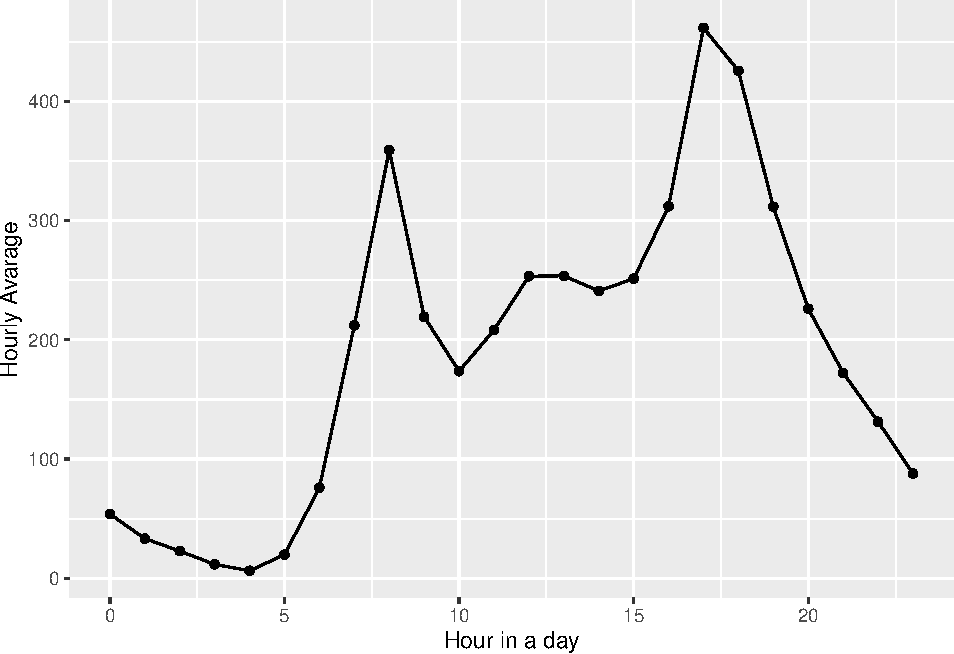
\includegraphics{_main_files/figure-latex/unnamed-chunk-23-1.pdf}
In this plot, x axis stands for the 24 hours in a single day. 0 is midnight and 10 is 10a.m., so on so forth.

Y is the average ridership of each hour throughout all days in this data.

We can see that the average ridership around morning rush hour and afternoon rush hour are 2 peaks. Also, it remains fairly high during daytime but swiftly decreases in the evening.

\hypertarget{plot-b}{%
\subsubsection{Plot B}\label{plot-b}}

\begin{Shaded}
\begin{Highlighting}[]
\NormalTok{workingday0\_b }\OtherTok{=}\NormalTok{ bikeshare }\SpecialCharTok{\%\textgreater{}\%} \FunctionTok{filter}\NormalTok{(workingday }\SpecialCharTok{==} \DecValTok{0}\NormalTok{) }\SpecialCharTok{\%\textgreater{}\%} \FunctionTok{group\_by}\NormalTok{(hr) }\SpecialCharTok{\%\textgreater{}\%} \FunctionTok{summarise}\NormalTok{(}\AttributeTok{avg =} \FunctionTok{mean}\NormalTok{(total)) }\SpecialCharTok{\%\textgreater{}\%} \FunctionTok{add\_column}\NormalTok{(}\AttributeTok{workingday =} \DecValTok{0}\NormalTok{)}
\NormalTok{workingday1\_b }\OtherTok{=}\NormalTok{ bikeshare }\SpecialCharTok{\%\textgreater{}\%} \FunctionTok{filter}\NormalTok{(workingday }\SpecialCharTok{==} \DecValTok{1}\NormalTok{) }\SpecialCharTok{\%\textgreater{}\%} \FunctionTok{group\_by}\NormalTok{(hr) }\SpecialCharTok{\%\textgreater{}\%} \FunctionTok{summarise}\NormalTok{(}\AttributeTok{avg =} \FunctionTok{mean}\NormalTok{(total)) }\SpecialCharTok{\%\textgreater{}\%} \FunctionTok{add\_column}\NormalTok{(}\AttributeTok{workingday =} \DecValTok{1}\NormalTok{)}
\NormalTok{tb\_b }\OtherTok{=} \FunctionTok{rbind}\NormalTok{(workingday0\_b, workingday1\_b)}
\NormalTok{tb\_b }\SpecialCharTok{\%\textgreater{}\%} \FunctionTok{ggplot}\NormalTok{(}\FunctionTok{aes}\NormalTok{(}\AttributeTok{x=}\NormalTok{hr,}\AttributeTok{y=}\NormalTok{avg)) }\SpecialCharTok{+} \FunctionTok{geom\_line}\NormalTok{()}\SpecialCharTok{+} \FunctionTok{geom\_point}\NormalTok{() }\SpecialCharTok{+} \FunctionTok{facet\_wrap}\NormalTok{(}\SpecialCharTok{\textasciitilde{}}\NormalTok{workingday) }\SpecialCharTok{+} \FunctionTok{labs}\NormalTok{(}\AttributeTok{x =} \StringTok{"Hour in a day"}\NormalTok{, }\AttributeTok{y =} \StringTok{"Hourly Avarage"}\NormalTok{)}
\end{Highlighting}
\end{Shaded}

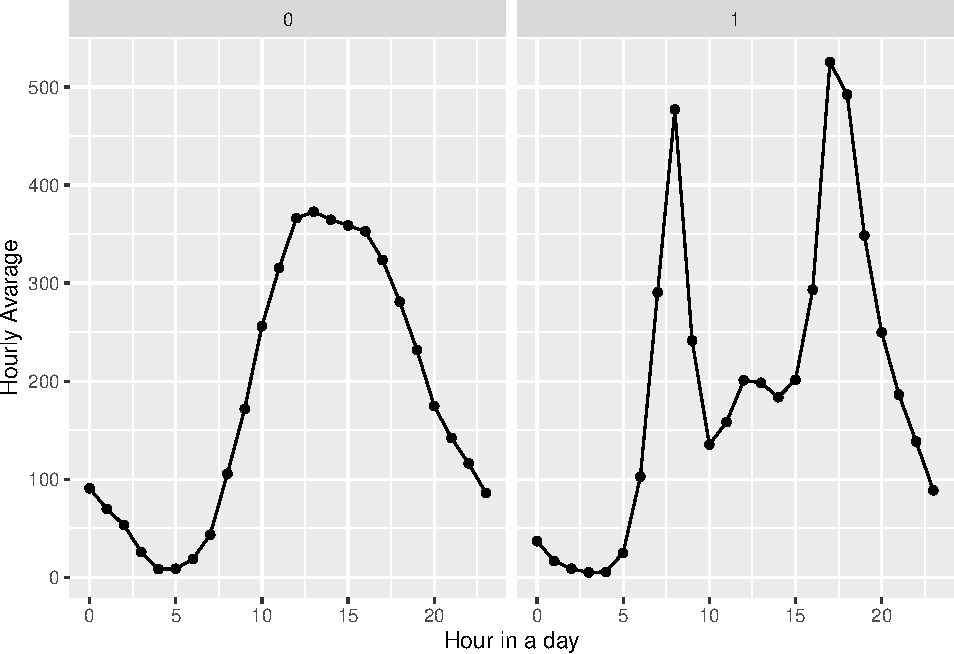
\includegraphics{_main_files/figure-latex/unnamed-chunk-24-1.pdf}
X and Y axis basically are the same as the plot A.

0 means weekends and holidays, while 1 means workdays. Workdays' pattern is pretty close to plot A and it complies with common sense. But non-holidays' pattern are quite different from Plot days, people tends to use bikes around noon till afternoon. I guess that people are likely to hang out during this time.

\hypertarget{plot-c}{%
\subsubsection{Plot C}\label{plot-c}}

\begin{Shaded}
\begin{Highlighting}[]
\NormalTok{workingday0\_c }\OtherTok{=}\NormalTok{ bikeshare }\SpecialCharTok{\%\textgreater{}\%} 
                \FunctionTok{filter}\NormalTok{(hr }\SpecialCharTok{==} \DecValTok{9}\NormalTok{) }\SpecialCharTok{\%\textgreater{}\%} 
                \FunctionTok{filter}\NormalTok{(workingday }\SpecialCharTok{==} \DecValTok{0}\NormalTok{) }\SpecialCharTok{\%\textgreater{}\%} 
                \FunctionTok{group\_by}\NormalTok{(weathersit) }\SpecialCharTok{\%\textgreater{}\%} 
                \FunctionTok{summarise}\NormalTok{(}\AttributeTok{avg =} \FunctionTok{mean}\NormalTok{(total)) }\SpecialCharTok{\%\textgreater{}\%} 
                \FunctionTok{add\_column}\NormalTok{(}\AttributeTok{workingday =} \DecValTok{0}\NormalTok{)}

\NormalTok{workingday1\_c }\OtherTok{=}\NormalTok{ bikeshare }\SpecialCharTok{\%\textgreater{}\%} 
                \FunctionTok{filter}\NormalTok{(hr }\SpecialCharTok{==} \DecValTok{9}\NormalTok{) }\SpecialCharTok{\%\textgreater{}\%} 
                \FunctionTok{filter}\NormalTok{(workingday }\SpecialCharTok{==} \DecValTok{1}\NormalTok{) }\SpecialCharTok{\%\textgreater{}\%} 
                \FunctionTok{group\_by}\NormalTok{(weathersit) }\SpecialCharTok{\%\textgreater{}\%} 
                \FunctionTok{summarise}\NormalTok{(}\AttributeTok{avg =} \FunctionTok{mean}\NormalTok{(total)) }\SpecialCharTok{\%\textgreater{}\%} 
                \FunctionTok{add\_column}\NormalTok{(}\AttributeTok{workingday =} \DecValTok{1}\NormalTok{)}

\NormalTok{tb\_c }\OtherTok{=} \FunctionTok{rbind}\NormalTok{(workingday0\_c, workingday1\_c)}
\NormalTok{tb\_c }\SpecialCharTok{\%\textgreater{}\%} \FunctionTok{ggplot}\NormalTok{(}\FunctionTok{aes}\NormalTok{(weathersit,}\AttributeTok{y=}\NormalTok{avg)) }\SpecialCharTok{+} \FunctionTok{geom\_bar}\NormalTok{(}\AttributeTok{stat=}\StringTok{\textquotesingle{}identity\textquotesingle{}}\NormalTok{, }\AttributeTok{fill=}\StringTok{"forest green"}\NormalTok{) }\SpecialCharTok{+} \FunctionTok{facet\_wrap}\NormalTok{(}\SpecialCharTok{\textasciitilde{}}\NormalTok{workingday) }\SpecialCharTok{+} \FunctionTok{labs}\NormalTok{(}\AttributeTok{x =} \StringTok{"Weather Situation"}\NormalTok{, }\AttributeTok{y =} \StringTok{"Avereage Ridership around 9AM"}\NormalTok{)}
\end{Highlighting}
\end{Shaded}

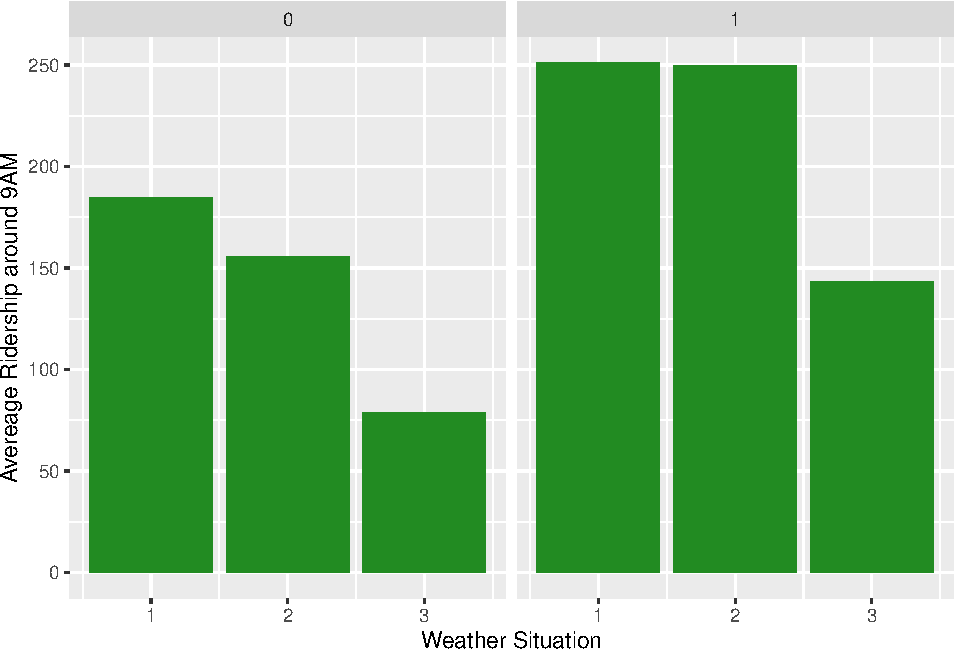
\includegraphics{_main_files/figure-latex/unnamed-chunk-25-1.pdf}
0 and 1 has the same meaning as Part B.

X axis means weather situation where 1 means sunny day, 2 means cloudy and misty day, and 3 means light snowy and light rainy day.

Y axis represents the avarage ridership around 9a.m.

So, in non-workdays, when the weather becomes cloudy, a few people may not go out riding bike because they might think that there will be potential rains. However, in workdays, almost all people will not change their original plan, which is getting a bike, just because of potential rains. They have to work!

  \bibliography{book.bib,packages.bib}

\end{document}
